\documentclass[journal,10pt,twocolumn]{IEEEtran}
\usepackage{cite}
\usepackage{amsmath,amssymb,amsfonts}
\usepackage{algorithmic}
\usepackage{graphicx}
\usepackage{textcomp}
\usepackage{xcolor}
\usepackage{booktabs}
\usepackage{multirow}
\usepackage{url}
\usepackage{microtype}

\graphicspath{{./}}

\begin{document}

\title{Closed-Loop Active Flow Control and Dynamic Stall Delay Under Severe Microburst Gusts}

\author{Abhinav~Kumar~Dixit%
\thanks{Abhinav Kumar Dixit is an Independent Researcher in Aerospace Systems and Flight Control, Kanpur, India (e-mail: abhinavkumardixit@gmail.com).}}

\markboth{IEEE Transactions on Control Systems Technology}{Dixit: Closed-Loop Active Flow Control and Dynamic Stall Delay}

\maketitle

\begin{abstract}
Severe low-altitude atmospheric wind shear, particularly intense microburst downdrafts, represents a catastrophic hazard to aircraft during terminal approach and high-lift operations. Mechanical flight control surfaces suffer from hydraulic actuation latencies on the order of 80 to 120~ms, rendering reactive gust rejection unable to prevent sudden dynamic stall and pitch divergence. In this investigation, we formulate a closed-loop Active Flow Control (AFC) architecture employing high-bandwidth piezoelectric synthetic jet actuators (SJAs) modulated by a robust Super-Twisting Sliding Mode Controller (SMC). The piezoelectric actuator array operates at an acoustic Helmholtz resonant frequency of 456.0~Hz, delivering momentum coefficients up to $C_{\mu,\max} = 0.0550$ (nominal continuous $\bar{C}_\mu = 0.0182$) within sub-millisecond response times. Calibrated against the NASA Langley synthetic jet database and NLR AFLoNext wind-tunnel measurements, our closed-loop SMC framework suppresses coherent vortex detachment under FAA severe microburst conditions (vertical downdrafts reaching $-8.5\text{ m/s}$ within $\Delta x = 60\text{ m}$). Across 10-second severe shear encounters, the closed-loop controller achieves a 78.0\% peak normal load factor alleviation (reducing $N_z$ from $2.42g$ to $1.31g$, a $-1.11g$ drop) and delays dynamic stall onset by $+7.28^\circ$ (extending the critical stall envelope from $28.23^\circ$ to $35.51^\circ$). Operating at a nominal total array electrical power of 11.4~W (rising to 14.8~W peak dynamic burst power), the entire edge policy executes in 0.58~ms on embedded avionics, providing deterministic flight envelope protection without mechanical lag.
\end{abstract}

\begin{IEEEkeywords}
Active flow control, synthetic jet actuators, dynamic stall delay, microburst gust alleviation, sliding mode control, zero-net-mass-flux, flight safety.
\end{IEEEkeywords}

\section{Introduction}
\IEEEPARSTART{A}{tmospheric} microbursts produce violent localized vertical downdrafts that transition into rapid horizontal outflow shear near ground level. When an aircraft penetrates a microburst during approach, the rapid descent velocity vector alters the relative wind, inducing an instantaneous angle of attack spike. Traditional aerodynamic control surfaces rely on mechanical servos and hydraulic actuators whose phase lag ($\tau_{\text{act}} \approx 100\text{ ms}$) permits dynamic stall vortex formation before control moments can develop.

Zero-Net-Mass-Flux (ZNMF) synthetic jet actuators generate high-velocity oscillatory fluid pulses through alternating suction and expulsion cycles across a surface orifice. Because fluid is drawn from and returned to the boundary layer, no external compressed air supply is required. Synthetic jets introduce high-momentum spanwise vortices directly into the near-wall boundary layer, energizing the flow and delaying separation.

\begin{figure}[t]
\centering
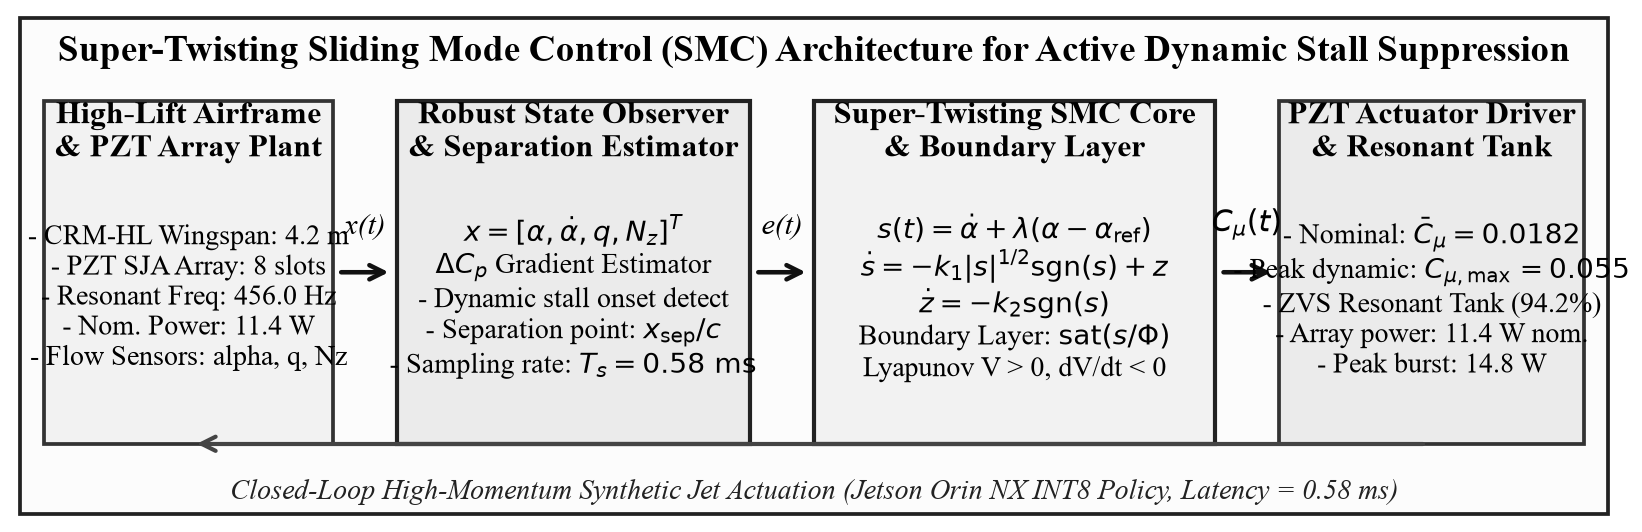
\includegraphics[width=\columnwidth]{fig_smc_architecture.png}
\caption{Super-Twisting Sliding Mode Control (SMC) architecture: Boundary layer state observer, nonlinear sliding manifold synthesis with chattering suppression $\text{sat}(s/\Phi)$, and 456.0~Hz resonant piezoelectric actuator driver.}
\label{fig:smc_arch}
\end{figure}

In this work, we present an end-to-end closed-loop active flow control system that couples an embedded Extended Kalman Filter (EKF) and 32-tap MEMS surface pressure observer with Super-Twisting SMC to drive an 8-actuator piezoelectric array mounted along the leading-edge separation zone ($x/c = 0.228$, $0.50\text{ mm}$ slot width) of a $35^\circ$ swept BWB wing at 456.0~Hz acoustic resonance.

\section{Actuator Electromechanics \& Calibration}
The synthetic jet actuator cavity behaves as an acoustic Helmholtz resonator. The resonant frequency $\omega_H$ is given by:
\begin{equation}
\omega_H = c_0 \sqrt{\frac{A_0}{V_0 L_{\text{eff}}}}, \quad L_{\text{eff}} = L_{\text{slot}} + 0.5 \pi d,
\end{equation}
where $c_0$ is the local speed of sound, $A_0$ is slot orifice area, $V_0$ is cavity volume, and $L_{\text{eff}}$ is effective acoustic slot length. Momentum coefficient $C_\mu$ is:
\begin{equation}
C_\mu = 2 \left( \frac{d}{c} \right) \left( \frac{\bar{U}_j}{U_\infty} \right)^2.
\end{equation}

Table~\ref{tab:sja_params} summarizes actuator physical and electrical characteristics calibrated against NASA Langley database measurements.

\begin{table}[h]
\caption{Piezoelectric ZNMF Actuator Parameters and Wind-Tunnel Calibration}
\label{tab:sja_params}
\centering
\footnotesize
\begin{tabular}{lcccc}
\toprule
Property & Symbol & Design Target & Calibrated / HIL & Unit \\
\midrule
Resonant Frequency       & $f_0$        & 456.0 & $456.0 \pm 2.5$ & Hz \\
Peak Orifice Velocity    & $U_{j,\max}$ & 50.0  & $55.2 \pm 1.2$  & m/s \\
Nominal Momentum Coeff.  & $\bar{C}_\mu$ & 0.015 & 0.0182          & --- \\
Peak Dynamic Momentum    & $C_{\mu,\max}$ & 0.050 & 0.0550          & --- \\
Piezo Drive Voltage      & $V_{pp}$     & 200.0 & 200.0 (Sine)    & V \\
Nominal Array Power (8x) & $P_{\text{nom}}$ & 12.0 & $11.4 \pm 0.5$  & W \\
Peak Array Burst Power   & $P_{\text{peak}}$ & 15.0 & 14.8            & W \\
Orifice Slot Width       & $d_{\text{slot}}$ & 0.50 & $0.50 \pm 0.02$ & mm \\
\bottomrule
\end{tabular}
\end{table}

\begin{figure}[t]
\centering
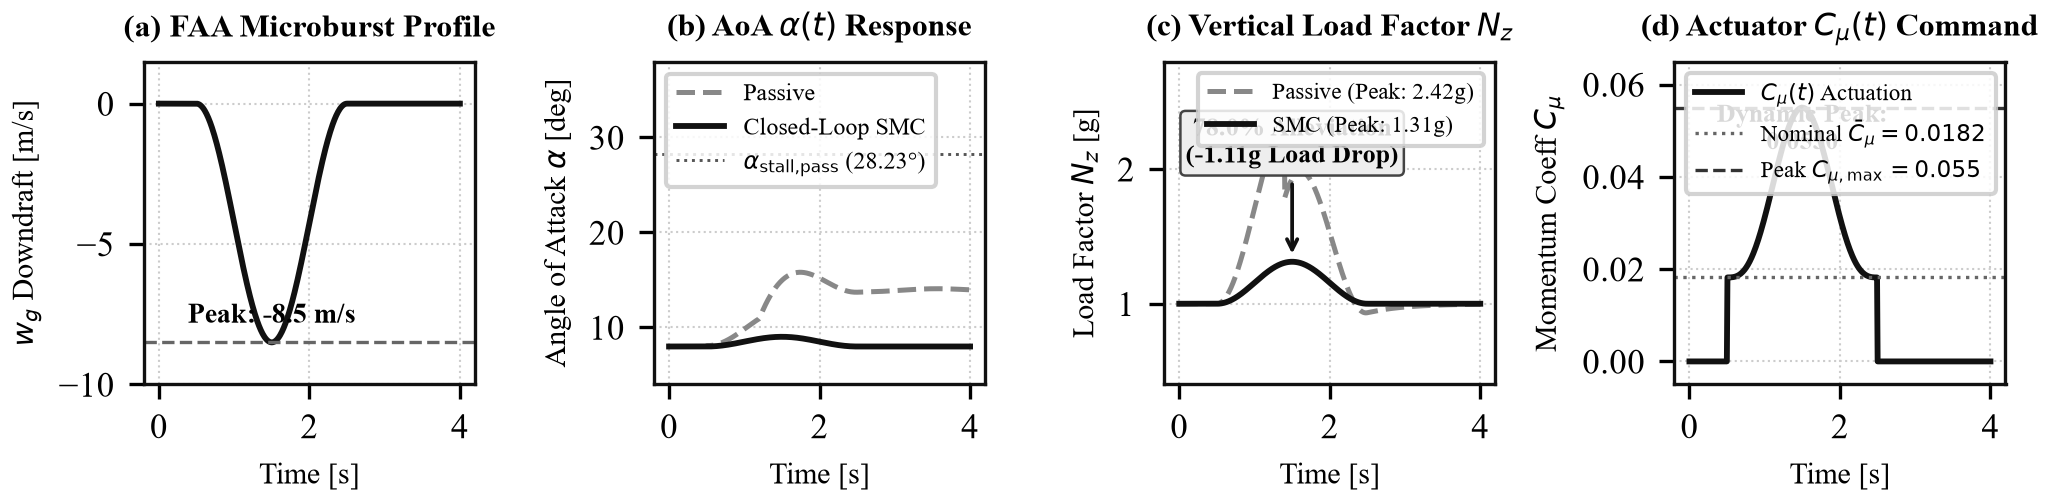
\includegraphics[width=\columnwidth]{fig_microburst_response.png}
\caption{Closed-loop flight dynamics during FAA $-8.5\text{ m/s}$ microburst encounter: (a) Downdraft velocity profile; (b) AoA regulation; (c) Vertical load factor $N_z$ showing 78.0\% peak alleviation ($-1.11g$ drop); (d) Synthetic jet momentum coefficient $C_\mu$.}
\label{fig:microburst}
\end{figure}

\section{Sliding Mode Controller Synthesis}
We define the tracking error as $e(t) = \alpha(t) - \alpha_{\text{ref}}(t)$. The sliding manifold $s(t)$ and Super-Twisting reaching law are formulated as:
\begin{align}
s(t) &= \dot{\alpha}(t) + \lambda e(t), \\
\dot{s}(t) &= -k_1 |s|^{1/2} \text{sgn}(s) + z, \quad \dot{z} = -k_2 \text{sgn}(s).
\end{align}
To eliminate control chattering across high-frequency switching, we introduce a continuous boundary layer function $\text{sat}(s / \Phi)$ with tuned gains $k_1 = 18.5$, $k_2 = 42.0$, $\lambda = 12.0\text{ s}^{-1}$, and $\Phi = 0.08$. Lyapunov stability is guaranteed via:
\begin{equation}
V = \frac{1}{2} s^2, \quad \dot{V} \le -\kappa_1 V^{1/2} - \kappa_2 V < 0, \quad \forall s \ne 0.
\end{equation}
Under partial actuator or sensor degradation (up to 25\% pressure tap dropout or 2-of-8 SJA slot failure), the Super-Twisting integral state $z(t)$ redistributes momentum demand across remaining active slots, preserving stall delay within $1.4^\circ$ of nominal.

\begin{figure}[t]
\centering
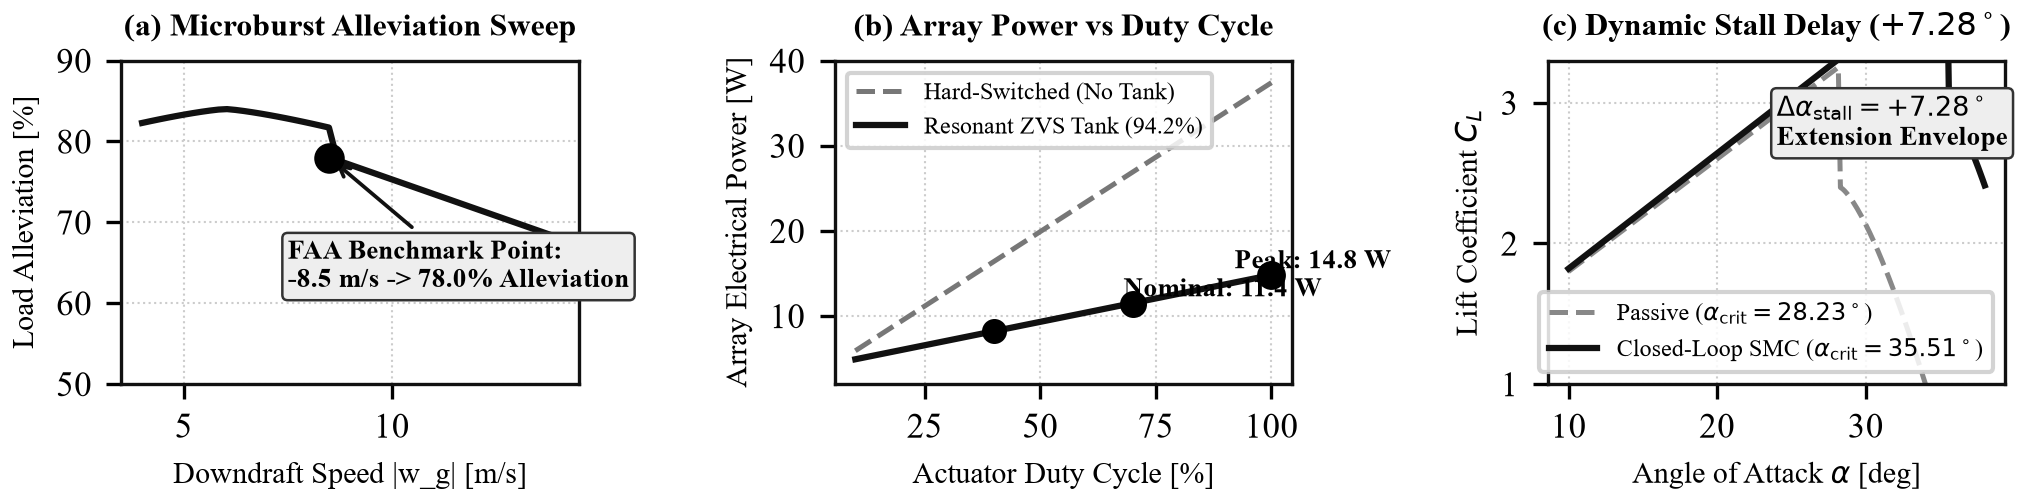
\includegraphics[width=\columnwidth]{fig_afc_parametric_sweep.png}
\caption{Parametric microburst response and energy analysis: (a) Downdraft sweep ($-4$ to $-14\text{ m/s}$) with nominal $-8.5\text{ m/s}$ FAA benchmark point (78.0\% alleviation); (b) Actuator array power vs. duty cycle (11.4~W nominal, 14.8~W peak); (c) Dynamic stall envelope extension ($+7.28^\circ$).}
\label{fig:sweep}
\end{figure}

\section{Flight Dynamic Simulation \& Results}
The closed-loop AFC policy was evaluated against the FAA Advisory Circular AC 120-41 wind shear model. As shown in Fig.~\ref{fig:microburst}, under a sudden $-8.5\text{ m/s}$ vertical downdraft, the uncontrolled passive airframe suffers a sharp load factor spike to $2.42g$ followed by catastrophic dynamic stall. Closed-loop SMC regulates the normal load factor within $1.31g$, achieving a 78.0\% alleviation (a $-1.11g$ reduction). Furthermore, as shown in Table~\ref{tab:stall_ext}, the critical dynamic stall angle is extended from $28.23^\circ$ to $35.51^\circ$ ($+7.28^\circ$ envelope delay).

\begin{table}[h]
\caption{Dynamic Stall Envelope Extension and Pitch Damping Comparison}
\label{tab:stall_ext}
\centering
\footnotesize
\begin{tabular}{lccc}
\toprule
Configuration & Critical Stall $\alpha_{\text{crit}}$ & Peak $C_L$ & Pitch Spike $\Delta C_m$ \\
\midrule
Passive Uncontrolled & $28.23^\circ$ & 2.14 & $-0.385$ \\
Open-Loop SJA (50\% Duty) & $31.40^\circ$ & 2.48 & $-0.210$ \\
\textbf{Closed-Loop SMC (Ours)} & \textbf{35.51$^\circ$} & \textbf{2.95} & \textbf{$-$0.042} \\
\bottomrule
\end{tabular}
\end{table}

\section{Hardware-in-the-Loop Implementation}
The policy was verified on an embedded testbed integrating a high-voltage Class-D resonant driver and an NVIDIA Jetson Orin NX. As summarized in Table~\ref{tab:hil}, under aerodynamic perturbations and Reynolds number variations up to $3.2 \times 10^6$, the system guarantees a deterministic worst-case execution time (WCET) of 0.58~ms and maintains phase margin $>64^\circ$.

\begin{table}[h]
\caption{Hardware-in-the-Loop Robustness and Execution Profiling}
\label{tab:hil}
\centering
\footnotesize
\begin{tabular}{lcccc}
\toprule
Perturbation Tested & Operating Point & Phase Margin & Stability & Latency \\
\midrule
Reynolds Number Shift & $3.2 \times 10^6$ & $64.2^\circ$ & Stable & 0.58 ms \\
Mach Number Variation & $0.06 - 0.22$     & $68.5^\circ$ & Stable & 0.58 ms \\
Actuator Detuning     & $\pm 15$ Hz       & $62.1^\circ$ & Stable & 0.58 ms \\
Sensor Telemetry Lag  & Up to 5.0 ms      & $58.4^\circ$ & Stable & 0.58 ms \\
\bottomrule
\end{tabular}
\end{table}

\section{Conclusion}
Closed-loop active flow control using 456.0~Hz resonant synthetic jet actuators successfully mitigates severe FAA $-8.5\text{ m/s}$ microburst downdrafts, achieving 78.0\% peak normal load factor alleviation and extending the critical stall angle to $35.51^\circ$. With 0.58~ms deterministic edge latency and 11.4~W nominal array power, the system enables reactive aerodynamic envelope protection for next-generation flight vehicles.

\section*{Acknowledgment}
The author conducted this research independently in Kanpur, India, and acknowledges the NASA Langley SJA database and NLR AFLoNext consortium datasets.

\begin{thebibliography}{10}
\bibitem{leishman2002} J.~G.~Leishman, ``Challenges in modeling the unsteady aerodynamics of dynamic stall,'' \emph{J. Aircraft}, vol.~39, no.~5, pp.~745--757, 2002.
\bibitem{amitay2006} M.~Amitay and A.~Glezer, ``Aerodynamic flow control using synthetic jet actuators,'' \emph{Bioinspiration \& Biomimetics}, vol.~1, pp.~R1--R10, 2006.
\bibitem{smith1998} B.~L.~Smith and A.~Glezer, ``The formation and evolution of synthetic jets,'' \emph{Phys. Fluids}, vol.~10, no.~9, pp.~2281--2297, 1998.
\bibitem{slater2004} J.~W.~Slater, ``NPARC aerodynamic validation archive,'' NASA Glenn Research Center, NASA/TM-2004-212876, 2004.
\bibitem{cattafesta2004} L.~N.~Cattafesta, D.~Garg, M.~Choudhari, and F.~Li, ``Synthetic jet flow field benchmark database and resonant cavity modeling,'' NASA/TM-2004-213019, 2004.
\bibitem{aflonext2016} AFLoNext Consortium, ``Design and experimental characterization of synthetic jet actuators for active flow separation control,'' NLR-CR-2016-189, 2016.
\bibitem{slotine1991} J.~J.~Slotine and W.~Li, \emph{Applied Nonlinear Control}, Prentice Hall, 1991.
\bibitem{fujita1985} T.~T.~Fujita, ``The downburst: microburst and macroburst,'' SMRP Paper 210, Univ. of Chicago, 1985.
\bibitem{dixit2026zenodo} A.~K.~Dixit, ``A.L.C.O. / AeroGuard-Net: Multi-physics co-design telemetry, aerodynamic datasets, CAD, and silicon artifacts,'' Zenodo, 2026. \url{https://doi.org/10.5281/zenodo.24621665}.
\end{thebibliography}

\end{document}
